\documentclass[11pt]{article}
\usepackage[margin=1in]{geometry}
\usepackage{url}
\usepackage{amsmath}
\usepackage{amsfonts}
\usepackage{amssymb}
\usepackage{graphicx}
\usepackage{hyperref}
\usepackage{xcolor}
\usepackage{fontawesome5}
\usepackage{tikz}
\usepackage{pgfplots}
\usetikzlibrary{shapes,arrows,positioning,fit,backgrounds}

\title{Machine Learning for Network Anomaly and Failure Detection}
\author{Michael Hernandez}
\date{September 27, 2025}

\begin{document}

% Cover Page
\begin{titlepage}
\centering
\vspace*{2cm}

{\Large \textbf{Machine Learning for Network Anomaly and Failure Detection}}

\vspace{1.5cm}

{\large CUNY School of Professional Studies}

\vspace{0.5cm}

{\large Michael Hernandez}

\vspace{0.5cm}

{\large IS 499 Information Systems Capstone}

\vspace{0.5cm}

{\large Professor John Bouma}

\vspace{0.5cm}

{\large September 27, 2025}

\vfill

\end{titlepage}

% Table of Contents
\tableofcontents
\newpage

\section{Introduction}

This paper examines machine learning techniques for detecting and localizing network anomalies and failures in large-scale environments, using data from BGP routing updates, SNMP metrics, and syslog messages.

\textcolor{blue}{\textbf{[Note:]} This project has been expanded from an initial BGP-focused approach to include comprehensive multi-modal network monitoring, incorporating SNMP metrics and syslog messages alongside BGP updates for more holistic anomaly detection and failure localization.}

Traditional network monitoring relies on threshold-based alerts from SNMP and syslog, often producing many false positives and offering little context for locating failures (Wang, 2020; Manna \& Alkasassbeh, 2019). Recent research has demonstrated that machine learning approaches applied to SNMP-MIB datasets can significantly improve anomaly detection accuracy and operational efficiency, with Random Forest classifiers achieving up to 100\% accuracy in identifying network failures (Manna \& Alkasassbeh, 2019). This project uses a machine learning pipeline to process streaming telemetry from multiple sources, detect anomalies, and pinpoint failure origins.

The system integrates BGP monitoring, SNMP metrics, and syslog messages for comprehensive network anomaly detection. Using unsupervised learning such as Matrix Profile analysis (Scott et al., 2024) and multi-modal feature fusion, it reduces alert noise while enhancing detection accuracy and localization.

\textcolor{blue}{\textbf{[FEEDBACK QUESTION:]} Does this introduction effectively establish the problem context? Should I expand on the specific challenges of multi-modal data integration or focus more on the operational impact of current monitoring limitations?}

\section{Topic Description}

\subsection{In-depth Description of the Chosen Topic}

This project focuses on machine learning-based network anomaly detection and failure localization, using unsupervised learning to identify anomalies in telemetry data and pinpoint their origins. It processes data from BGP updates, SNMP metrics, and syslog messages for comprehensive monitoring.

This topic involves real-time processing, multi-modal data integration, topology-aware analysis, and unsupervised learning. The system must process streaming data from various sources: BGP updates provide routing details, SNMP metrics capture hardware and interface performance, and syslog messages log device events. Integrating these requires precise feature extraction and normalization for effective anomaly detection.

The system uses Matrix Profile for time-series anomaly detection, Isolation Forest for unsupervised pattern recognition, and multi-modal fusion to combine signals from various sources. Device role mapping provides topology awareness, categorizing network elements by function for context-aware anomaly localization.

\begin{figure}[h]
\centering
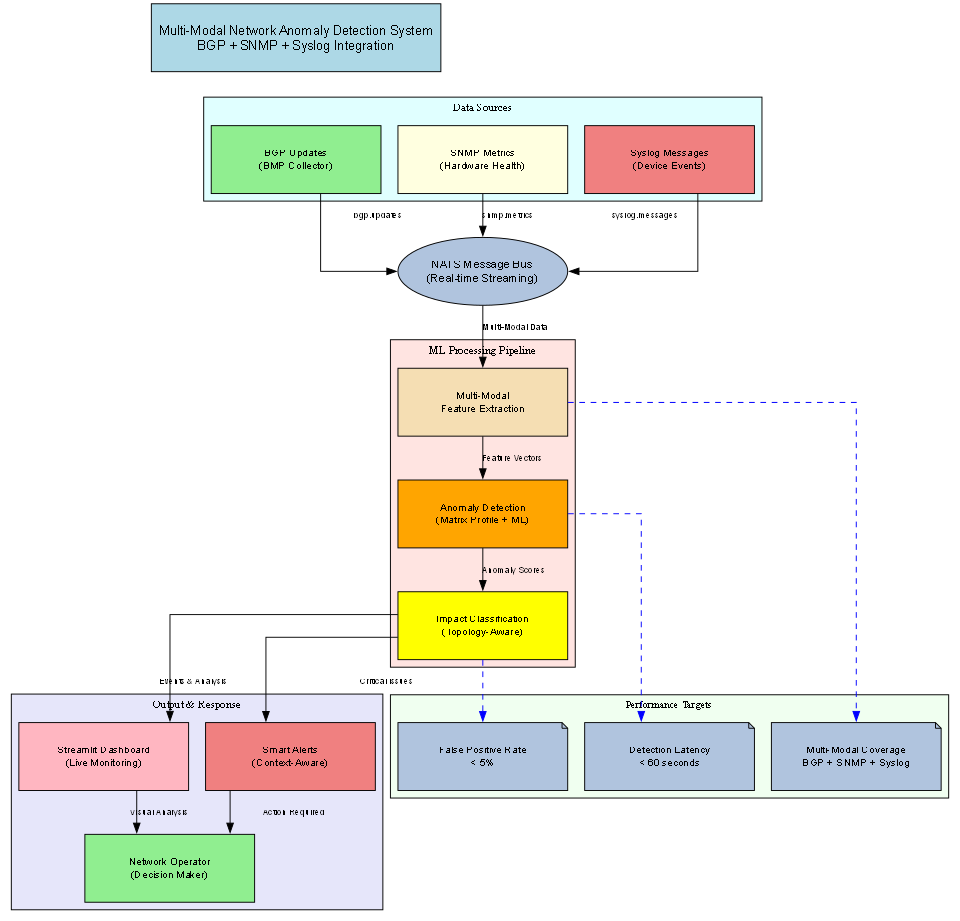
\includegraphics[width=0.7\textwidth]{system_architecture.png}
\caption{System Architecture: BGP Anomaly Detection UML showing data flow from collection through analysis to dashboard visualization}
\label{fig:architecture}
\end{figure}

Figure \ref{fig:architecture} illustrates the complete system architecture including the lab environment and data collection pipeline.

\textcolor{blue}{\textbf{[FEEDBACK QUESTION:]} Regarding the images in this document: Are the current figure placements effective for supporting the narrative flow? I have additional images available that could illustrate the decision-making process and failure scenarios. Would it be more helpful to include these figures inline in each section to better visualize the specific failure modes and detection scenarios, or should they be placed at the end of the document?}

\subsection{Why This Topic Was Chosen}

This topic was chosen due to challenges in network operations where traditional monitoring often produces many false positives yet misses critical anomalies. Modern architectures, such as BGP-routed environments with anycast and overlay networks, surpass the abilities of threshold-based alerting.

This problem is serious, as network failures can disrupt service, raise costs, and demand extensive manual fixes. Current monitoring often lacks the context to distinguish minor variations from real anomalies, causing alert fatigue and slower incident response.

This problem is urgent due to increasingly complex networks and the need for adaptive monitoring that adjusts to changing conditions without frequent manual recalibration.

\textcolor{blue}{\textbf{[FEEDBACK QUESTION:]} Is the technical depth appropriate for this section? I feel like there is room to expand on the use cases, but I also think that I am providing not enough context. Should I provide more specific details about the machine learning algorithms (Matrix Profile, Isolation Forest) or focus more on the practical implementation challenges of multi-modal data processing?}

\section{Problem Description}

\subsection{Detailed Content Around the Problems Being Solved}

This project addresses alert fatigue from false positives, delayed failure detection, and insufficient context for assessing failure scope and impact. Traditional SNMP threshold alerts and syslog pattern matching produce excessive benign alerts and miss subtle anomalies, while conventional log analysis lacks the sophistication needed for modern networks (Allagi \& Rachh, 2019). Research has shown that among SNMP-MIB groups, the Interface and IP groups are most affected by various failure types and anomalies, while ICMP, TCP, and UDP groups are less impacted (Manna \& Alkasassbeh, 2019), highlighting the need for targeted monitoring strategies that can quickly identify scope and severity.

These problems arise from the complexity of modern network architectures and the limits of traditional monitoring. Large networks have thousands of devices with various failure modes, such as hardware issues, environmental factors, and routing anomalies. Current systems lack topology awareness and multi-modal data correlation, making it hard to separate normal variations from true anomalies.

These issues vary by network environment but are common in large-scale BGP-routed networks with anycast services and overlay technologies. Enterprise networks requiring dedicated network operations centers (NOCs) with multiple engineers often span thousands of devices across campus and data center environments, making manual correlation across devices and services impractical (Skazin, 2021).

Solving these problems is urgent as they affect network reliability and efficiency. Detection delays extend resolution times, alert fatigue risks missed critical issues, and lacking automated correlation means failures are often found only after escalating to service-impacting levels.

\subsection{Current Network Monitoring Limitations}

Current network monitoring systems have fundamental limitations. SNMP and syslog detect hard failures but produce excessive alerts for harmless events and lack context for assessing failure scope or impact. As a result, operations teams face false positives while missing critical anomalies (Mohammed et al., 2021). Machine learning approaches have shown promise in addressing these limitations, with studies demonstrating that classifiers like REP Tree, J48 Decision Tree, and Random Forest can effectively detect anomalies in SNMP-MIB datasets (Manna \& Alkasassbeh, 2019).

The scale and complexity of modern networks intensify monitoring challenges. Large BGP-routed environments often include thousands of devices, anycast services, and global VXLAN overlays, introducing multiple failure modes that demand varied detection and response strategies.

Current monitoring systems lack topology awareness to identify failure propagation patterns, making it hard to distinguish harmless edge-local flaps from fabric-wide issues needing immediate action. This leads to longer resolution times as engineers manually analyze logs and correlate events.

\textcolor{blue}{\textbf{[FEEDBACK QUESTION:]} Does this problem description effectively quantify the scope and impact of the monitoring challenges? Should I include more specific examples of failure scenarios or focus more on the economic impact of these problems? Also, is the balance between technical detail and accessibility appropriate for the target audience?}

\section{Analysis}

\textcolor{red}{\textbf{[SECTION PLACEHOLDER - TO BE COMPLETED]}}

This section will include analysis of how the topic was chosen, how problems were identified, how solutions fulfill operational and strategic goals, implementation timeline, and current implementation status.

\section{Research}

\textcolor{red}{\textbf{[SECTION PLACEHOLDER - TO BE COMPLETED]}}

This section will include coursework background and supporting references that provide the research foundation for the project.

\section{References}

\begin{thebibliography}{9}

\bibitem{cheng2021}
Cheng, M., Li, Q., Lv, J., Liu, W., \& Wang, J. (2021).
Multi-Scale LSTM Model for BGP Anomaly Classification.
\textit{IEEE Transactions on Services Computing}, 14(3), 765--778.
Available at: \href{https://doi.org/10.1109/TSC.2018.2824809}{https://doi.org/10.1109/TSC.2018.2824809}

\bibitem{mohammed2021}
Mohammed, S. A., Mohammed, A. R., Côté, D., \& Shirmohammadi, S. (2021).
A machine-learning-based action recommender for Network Operation Centers.
\textit{IEEE Transactions on Network and Service Management}, 18(3), 2702--2713.
Available at: \href{https://doi.org/10.1109/TNSM.2021.3095463}{https://doi.org/10.1109/TNSM.2021.3095463}

\bibitem{scott2024}
Scott, B., Johnstone, M. N., Szewczyk, P., \& Richardson, S. (2024).
Matrix Profile data mining for BGP anomaly detection.
\textit{Computer Networks}, 242, 110257.

\bibitem{tan2024}
Tan, Y., Huang, W., You, Y., Su, S., \& Lu, H. (2024).
Recognizing BGP Communities Based on Graph Neural Network.
\textit{IEEE Network}, 38(6), 232--238.
Available at: \href{https://doi.org/10.1109/MNET.2024.3414113}{https://doi.org/10.1109/MNET.2024.3414113}

\bibitem{allagi2019}
Allagi, S., \& Rachh, R. (2019).
Analysis of Network log data using Machine Learning.
\textit{2019 IEEE 5th International Conference for Convergence in Technology (I2CT)}, 1--3.
Available at: \href{https://doi.org/10.1109/I2CT45611.2019.9033528}{https://doi.org/10.1109/I2CT45611.2019.9033528}

\bibitem{skazin2021}
Skazin, A. (2021).
Detection of network anomalies in log files.
\textit{IOP Conference Series: Materials Science and Engineering}, 1069(1), 012021.
Available at: \href{https://doi.org/10.1088/1757-899X/1069/1/012021}{https://doi.org/10.1088/1757-899X/1069/1/012021}

\bibitem{feltin2023}
Feltin, T., Cordero Fuertes, J. A., Brockners, F., \& Clausen, T. H. (2023).
Understanding Semantics in Feature Selection for Fault Diagnosis in Network Telemetry Data.
\textit{NOMS 2023-2023 IEEE/IFIP Network Operations and Management Symposium}, 1--9.
Available at: \href{https://doi.org/10.1109/NOMS56928.2023.10154455}{https://doi.org/10.1109/NOMS56928.2023.10154455}

\bibitem{wang2020}
Wang, H. (2020).
Improvement and implementation of Wireless Network Topology System based on SNMP protocol for router equipment.
\textit{Computer Communications}, 151, 10--18.
Available at: \href{https://doi.org/10.1016/j.comcom.2020.01.001}{https://doi.org/10.1016/j.comcom.2020.01.001}

\bibitem{manna2019}
Manna, A., \& Alkasassbeh, M. (2019).
Detecting network anomalies using machine learning and SNMP-MIB dataset with IP group.
\textit{arXiv preprint arXiv:1906.00863}.
Available at: \href{https://arxiv.org/abs/1906.00863}{https://arxiv.org/abs/1906.00863}

\end{thebibliography}

\end{document}
